\documentclass{article}
\usepackage[a4paper, total={7in, 9in}]{geometry}
\usepackage{multicol}
\usepackage{blindtext}
\usepackage{caption}
\PassOptionsToPackage{hyphens}{url}\usepackage{hyperref}


\title{Course Project: Exploring Batch Normalization}
\author{Zony Yu}
\date{Dec 1, 2021}

\usepackage{mathbbol}
\usepackage{amsmath}
\usepackage{amssymb}
\usepackage{graphicx}
\usepackage{subfig}
\graphicspath{{assets/}}

\begin{document}
100%
\begin{multicols}{2}









\section*{1.0: Introduction}
In the field of supervised learning, a mathematical model is fit to 
a training dataset using various optimization schemes such that the model 
can be used to make predictions on unseen data. However, 
due to the nature of most training data, optimization is often made more 
difficult. In many multivariate learning problems, the input features are
often on completely different scales. This leads to a highly eccentric cost
function where gradients with respect to certain weights are much steeper
than with respect to other weights. This requires learning rates to 
be very small in order not to overshoot in any dimension.

To solve this problem, many feature scaling techniques were developed to ensure
that all input features are roughly on the same scale. One example is \textbf{standardization}
where raw features are processed by subtracting by the mean of the data and 
scaling by the standard deviation:

\begin{equation}
    \hat{x}_j^{(i)} = {x^{(i)}_j - \mu_j \over \sigma_j} \notag
\end{equation}

Here, each training feature $j$ of training example $i$ is standardized separately, 
where $\begin{aligned}
    \mu_j = {1\over M}\sum_i x^{(i)}_j
\end{aligned}$ and $\begin{aligned}
    \sigma^2_j = {1\over M}\sum_i (x^{(i)}_j - \mu_j)^2
\end{aligned}$. Note that $M$ represents the number of examples in the 
training set. This method is often considered to be a sufficient solution 
for linear models to mitigate highly eccentric cost functions. However, 
standardization is much less effective for neural networks.

To understand its shortcomings when applied to neural networks, consider
the following example: suppose we model the linear transformation 
of a single layer within the NN:

\begin{equation}
    \textbf{z} = \textbf{Wx} + \textbf{b} \notag
\end{equation}

We may assume that $\textbf{x} \sim \mathcal{N}(0, 1)$, however this by no means
guarantee that $\textbf{z} \sim \mathcal{N}(0, 1)$. This is problematic because 
$\textbf{z}$ (after passing it through a nonlinearity) becomes the input to
the next layer. A non-standardized $\textbf{z}$ introduces different
behaviours on the succeeding layer's inputs depending on the nonlinearity 
used -- ReLU functions will preserve all features of $\textbf{z}$ that are positive,
of which features could be on vastly different scales,
and Sigmoid and Tanh functions will saturate on certain features of $\textbf{z}$
if the magnitudes are large.










\subsection*{1.1: Batch Normalization}
In the 2015 paper ``\textit{Batch Normalization: Accelerating Deep Network Training 
by Reducing Internal Covariate Shift}'' (S. Ioffe, C. Szegedy, 2015), the researchers
propose a method to standardize the weighted sum of each layer, ensuring that their
distributions remain stable during training. This elimination of ``\textit{Internal Covariate Shift}''allows the use of much larger learning
rates without the gradients diverging, thus greatly accelerating convergence.

Since Batch Normalization (BN) is applied layer-wise in a neural network, 
there needs to be a way to backpropagate through each BN layer, which 
was not needed in prior linear models using input feature standardization.
While the aforementioned paper presented the equations for the backpropagated
gradients, in this paper we will discuss the derivation of backpropagation
in greater detail. This paper will also present qualitative and quantitative
differences between experiments carried out on neural networks with 
and without BN.








\section*{2.0: Formulation}

Batch Normalization applies feature standardization to the weighted sum of 
each layer, which then the normalized outputs are fed into the nonlinearity.
A concrete description is shown below:

\begin{equation}
    \textbf{z}^{(i)} = \textbf{W}\textbf{x}^{(i)} \notag
\end{equation}
\begin{equation}
    \hat{\textbf{y}}^{(i)} = \text{BN}(\textbf{z}^{(i)}) \notag
\end{equation}
\begin{equation}
    \textbf{a}^{(i)} = f(\hat{\textbf{y}}^{(i)}) 
\end{equation}

In the above equations, we use $\textbf{x}$ to denote the inputs to the layer, 
$\textbf{z}$ to denote the output of the weighted sum, 
$\hat{\textbf{y}}$ to denote the standardized weighted sum,
$\textbf{a}$ to denote the nonlinearity output, and $(i)$ represents index 
of the training element.
It's worth mentioning that a common area of contention is the placement 
of BN with respect to the activation function. This topic by itself 
can form an entire area of research, so for this paper we will stick with the 
implementation of the original 2015 paper, placing BN \textbf{before} the nonlinearity.

Applying feature standardization on the weighted sum, we get the following:

\begin{equation}
    \hat{\textbf{z}}^{(i)} = {\textbf{z}^{(i)} - \boldsymbol{\mu}\over \sqrt{\boldsymbol{\sigma}^2 + \epsilon}} 
\end{equation}

Note that we add a small $\epsilon$ in the denominator for numeric stability.
Here, $\boldsymbol{\mu} = \text{E}[\textbf{z}]$ and 
$\boldsymbol{\sigma}^2 = \text{Var}[\textbf{z}]$. BN computes the standardization
of every example within a batch, so we should specify that $\textbf{z}$
represents the output of the weighted sum with dimensions $M_{\text{batch}} \times N_x$,
Where $M_{\text{batch}}$ represents the batch size and $N_x$ represents the 
number of features in $\textbf{x}$.

Once we get the standardized output 
$\hat{\textbf{z}}^{(i)}$, we observe that directly using this result can limit 
the hypothesis capacity of the neural network. Suppose we compare two
weighted sums: $\textbf{z}^{(i)} = \textbf{Wx}^{(i)}$ and $\textbf{z}'^{(i)} = \textbf{Wx}^{(i)} + \textbf{b}$.
We can compute the means...

\begin{equation}
    \boldsymbol{\mu} = \text{E}[\textbf{z}] \notag
\end{equation}
\begin{equation}
    \boldsymbol{\mu}' = \text{E}[\textbf{z}'] = \text{E}[\textbf{z} + \textbf{b}] = \boldsymbol{\mu} + \textbf{b} \notag
\end{equation}

... As well as the variances:

\begin{equation}
    \boldsymbol{\sigma}^2 = \text{E}[\textbf{z} - \boldsymbol{\mu}]^2\notag
\end{equation}
\begin{equation}
    \boldsymbol{\sigma'}^2 = \text{E}[\textbf{z}' - \boldsymbol{\mu'}]^2\notag
\end{equation}
\begin{equation}
     = \text{E}[\textbf{z} + \textbf{b} - \boldsymbol{\mu} - \textbf{b}]^2\notag
\end{equation}
\begin{equation}
    = \boldsymbol{\sigma}^2 \notag
\end{equation}


We can then show that:

\begin{equation}
    \hat{\textbf{z}}'^{(i)} = {\textbf{z}'^{(i)} - \boldsymbol{\mu}' \over \sqrt{\boldsymbol{\sigma}^2 + \epsilon}} \notag
\end{equation}
\begin{equation}
    = {\textbf{z}^{(i)} + \textbf{b} - \boldsymbol{\mu} - \textbf{b} \over \sqrt{\boldsymbol{\sigma}^2 + \epsilon}} \notag
\end{equation}
\begin{equation}
    = \hat{\textbf{z}}^{(i)} \notag
\end{equation}

Here we observe that standardizing the weighted sum will ignore the bias
term. BN can be made more flexible by scaling the normalized sum and 
reintroducing the bias term:

\begin{equation}
    \hat{y}_j^{(i)} = \gamma_j \hat{z}_j^{(i)} + \beta_j \notag
\end{equation}
\begin{equation}
    \hat{\textbf{y}}^{(i)} = \boldsymbol{\gamma} \odot \hat{\textbf{z}}^{(i)} + \boldsymbol{\beta} 
\end{equation}

The rescaling factor $\boldsymbol{\gamma}$ and bias term $\boldsymbol{\beta}$ are 
parameters learnable through backpropagation. One example of the improved
flexibility is the ability to learn the identity function. Suppose $\boldsymbol{\gamma} = \sqrt{\boldsymbol{\sigma}^2 + \epsilon}$
and $\boldsymbol{\beta} = \boldsymbol{\mu}$, then we observe that $\hat{\textbf{y}}^{(i)} = \textbf{z}^{(i)}$.







\subsection*{2.1: Backpropagation}

In the beginning of \textbf{section 2.0}, we formulated the order of which
operations are performed in forward propagation through a single layer (1). 
Backpropagation involves propagating the gradients in the reverse order, which
requires computing several gradients of BN. This includes calculating 
$\begin{aligned}
    {\partial J \over \partial \textbf{z}^{(i)}}
\end{aligned}$ for the $i^{\text{th}}$ input to BN, as well as $\begin{aligned}
    {\partial J \over \partial \boldsymbol{\gamma}}, {\partial J \over \partial \boldsymbol{\beta}}
\end{aligned}$ to learn the scaling and shifting parameters.

We will refer extensively to \textit{Figure 2.1.0} in the appendix 
to explain the process. This dependence graph shows the relations between 
each variable. For example, $J$ directly dependent on all $\hat{\textbf{y}}^{(i)}, 1 \leq i \leq M$.
The three bolded vectors points to all variables that $\textbf{z}^{(i)}$ has 
direct contributions to, namely $\boldsymbol{\mu}, \boldsymbol{\sigma}^2$, 
and $\hat{\textbf{z}}^{(i)}$. Therefore, we can formulate the gradients from here.
Note that for this portion of the paper, all all multiplication operations
are assumed to be pointwise rather than matrix, in order to reduce clutter.
Also, it's worth mentioning that $\boldsymbol{\gamma}$ and $\boldsymbol{\beta}$
are intentionally left out of this particular diagram for the same reason.

\begin{equation}
    {\partial J \over \partial \textbf{z}^{(i)}} = {\partial J \over \partial \hat{\textbf{z}}^{(i)}}
    {\partial \hat{\textbf{z}}^{(i)} \over \partial \textbf{z}^{(i)}}
     + {\partial J \over \partial \boldsymbol{\sigma}^2} 
     {\partial \boldsymbol{\sigma}^2 \over \partial \textbf{z}^{(i)}}
     + {\partial J \over \partial \boldsymbol{\mu}}
     {\partial \boldsymbol{\mu} \over \partial \textbf{z}^{(i)}}
\end{equation}

Starting from the first term, we first compute $\begin{aligned}
    {\partial J \over \partial \hat{\textbf{z}}^{(i)}}
\end{aligned}$:

\begin{equation}
    {\partial J \over \partial \hat{\textbf{z}}^{(i)}} = 
    {\partial J \over \partial \hat{\textbf{y}}^{(i)}} 
    {\partial \hat{\textbf{y}}^{(i)} \over \partial \hat{\textbf{z}}^{(i)}} \notag
\end{equation}

Referring to equation (3), 

\begin{equation}
    {\partial \hat{\textbf{y}}^{(i)} \over \partial \hat{\textbf{z}}^{(i)}} = \boldsymbol{\gamma} \notag
\end{equation}

Therefore, 

\begin{equation}
    {\partial J \over \partial \hat{\textbf{z}}^{(i)}} = 
    {\partial J \over \partial \hat{\textbf{y}}^{(i)}} \boldsymbol{\gamma} \notag
\end{equation}

Referring to equation (2), we can compute $\begin{aligned}
    {\partial \hat{\textbf{z}}^{(i)} \over \partial \textbf{z}^{(i)}}
\end{aligned}$:

\begin{equation}
    {\partial \hat{\textbf{z}}^{(i)} \over \partial \textbf{z}^{(i)}} = 
    {1 \over \sqrt{\boldsymbol{\sigma}^2 + \epsilon}} \notag
\end{equation}

The first term of equation (4) can be put together:

\begin{equation}
    {\partial J \over \partial \hat{\textbf{z}}^{(i)}}
    {\partial \hat{\textbf{z}}^{(i)} \over \partial \textbf{z}^{(i)}} = {\partial J \over \partial \hat{\textbf{y}}^{(i)}}
    \boldsymbol{\gamma} 
    {1 \over \sqrt{\boldsymbol{\sigma}^2 + \epsilon}} 
\end{equation}

Moving onto the second term, we compute $\begin{aligned}
    {\partial J \over \partial \boldsymbol{\sigma}^2}
\end{aligned}$. Note that $J$'s dependency on $\boldsymbol{\sigma}^2$
is split among many paths, so the gradient through each path must be
accounted for.
\begin{equation}
    {\partial J \over \partial \boldsymbol{\sigma}^2} = 
    \sum_{m = 1}^M {\partial J \over \partial \hat{\textbf{y}}^{(m)}} 
    {\partial \hat{\textbf{y}}^{(m)} \over \partial \hat{\textbf{z}}^{(m)}}
    {\partial \hat{\textbf{z}}^{(m)} \over \partial \boldsymbol{\sigma}^2} \notag
\end{equation}

Recall that $\begin{aligned}
    {\partial \hat{\textbf{y}}^{(m)} \over \partial \hat{\textbf{z}}^{(m)}} = \boldsymbol{\gamma}
\end{aligned}$. Now we calculate $\begin{aligned}
    {\partial \hat{\textbf{z}}^{(m)} \over \partial \boldsymbol{\sigma}^2} 
\end{aligned}$, referring to equation (2):

\begin{equation}
    {\partial \hat{\textbf{z}}^{(m)} \over \partial \boldsymbol{\sigma}^2} =
    -{1\over 2} (\textbf{z}^{(m)} - \boldsymbol{\mu}) (\boldsymbol{\sigma}^2 + \epsilon)^{-3/2} \notag
\end{equation}

Now we can complete $\begin{aligned}
    {\partial J \over \partial \boldsymbol{\sigma}^2}:
\end{aligned}$

\begin{equation}
    {\partial J \over \partial \boldsymbol{\sigma}^2} = -{1\over 2}
    \sum_{m = 1}^M {\partial J \over \partial \hat{\textbf{y}}^{(m)}} 
    \boldsymbol{\gamma}
    (\textbf{z}^{(m)} - \boldsymbol{\mu}) (\boldsymbol{\sigma}^2 + \epsilon)^{-3/2}
\end{equation}

We will now compute the second half of the second term in equation (4), 
namely $\begin{aligned}
    {\partial \boldsymbol{\sigma}^2 \over \partial \textbf{z}^{(i)}}
\end{aligned}$. From the dependencies graph we 
note that there are two paths that lead from $\textbf{z}^{(i)}$ to 
$\boldsymbol{\sigma}^2$, so the gradient must account for both contributions.
The point-wise variance $\boldsymbol{\sigma}^2$ is 
represented by the following equation:

\begin{equation}
    \boldsymbol{\sigma}^2 = {1\over M} 
    \sum_{m = 1}^M (\textbf{z}^{(m)} - \boldsymbol{\mu})^2
\end{equation}

And below is the gradient $\begin{aligned}
    {\partial \boldsymbol{\sigma}^2 \over \partial \textbf{z}^{(i)}}
\end{aligned}$:

\begin{equation}
    {\partial \boldsymbol{\sigma}^2 \over \partial \textbf{z}^{(i)}} = 
    \bigg[{\partial \boldsymbol{\sigma}^2 \over \partial \textbf{z}^{(i)}} \bigg]_{\text{Direct}}
    + {\partial \boldsymbol{\sigma}^2 \over \partial \boldsymbol{\mu}}
    {\partial \boldsymbol{\mu} \over \partial \textbf{z}^{(i)}}
\end{equation}

Here $\begin{aligned}
    \bigg[{\partial \boldsymbol{\sigma}^2 \over \partial \textbf{z}^{(i)}} \bigg]_{\text{Direct}}
\end{aligned}$ is the gradient resulting from the direct contribution of
$\textbf{z}^{(i)}$ to $\boldsymbol{\sigma}^2$, and the second term represents
the contribution of $\textbf{z}^{(i)}$ chained through $\boldsymbol{\mu}$.
First, we compute $\begin{aligned}
    \bigg[{\partial \boldsymbol{\sigma}^2 \over \partial \textbf{z}^{(i)}} \bigg]_{\text{Direct}}
\end{aligned}$ from equation (7):

\begin{equation}
    \bigg[{\partial \boldsymbol{\sigma}^2 \over \partial \textbf{z}^{(i)}} \bigg]_{\text{Direct}} =
    {2 \over M} (\textbf{z}^{(i)} - \boldsymbol{\mu}) \notag
\end{equation}

Now we can compute the second term of equation (8), starting with 
$\begin{aligned}
    {\partial \boldsymbol{\sigma}^2 \over \partial \boldsymbol{\mu}}
\end{aligned}$:

\begin{equation}
    {\partial \boldsymbol{\sigma}^2 \over \partial \boldsymbol{\mu}} = 
    -{2 \over M} \sum_{m=1}^M (\textbf{z}^{(m)} - \boldsymbol{\mu}) \notag
\end{equation}

Then, we compute $\begin{aligned}
    {\partial \boldsymbol{\mu} \over \partial \textbf{z}^{(i)}}
\end{aligned}$, knowing that the pointwise mean $\boldsymbol{\mu}$ is represented by the equation $\begin{aligned}
    \boldsymbol{\mu} = {1\over M} \sum_{m=1}^M\textbf{z}^{(m)}
\end{aligned}$:

\begin{equation}
    {\partial \boldsymbol{\mu} \over \partial \textbf{z}^{(i)}} = 
    {1\over M} 
\end{equation}

Now, we can complete equation (8) by piecing together the gradients 
we just calculated:

\begin{equation}
    {\partial \boldsymbol{\sigma}^2 \over \partial \textbf{z}^{(i)}} = 
    {2 \over M} (\textbf{z}^{(i)} - \boldsymbol{\mu})
    -{2 \over M^2} \sum_{m=1}^M (\textbf{z}^{(m)} - \boldsymbol{\mu}) \notag
\end{equation}

Combining equation (8), we complete the second term of equation (4).
In other words, we computed the change in cost $J$ with respect of 
$\textbf{z}^{(i)}$ chaining through $\boldsymbol{\sigma}^2$.

$$
\begin{aligned}
    {\partial J \over \partial \boldsymbol{\sigma}^2} 
    {\partial \boldsymbol{\sigma}^2 \over \partial \textbf{z}^{(i)}} = 
    \bigg[
    -{1\over 2}
    \sum_{m = 1}^M {\partial J \over \partial \hat{\textbf{y}}^{(m)}} 
    \boldsymbol{\gamma}
    (\textbf{z}^{(m)} - \boldsymbol{\mu}) (\boldsymbol{\sigma}^2 + \epsilon)^{-3/2} \bigg]\\
    \bigg[{2 \over M} (\textbf{z}^{(i)} - \boldsymbol{\mu})
    -{2 \over M^2} \sum_{m=1}^M (\textbf{z}^{(m)} - \boldsymbol{\mu})\bigg]
\end{aligned}
$$
    
$$ \begin{aligned}
    = {2 \over M} (\textbf{z}^{(i)} - \boldsymbol{\mu}) \bigg[
    -{1\over 2}
    \sum_{m = 1}^M {\partial J \over \partial \hat{\textbf{y}}^{(m)}} 
    \boldsymbol{\gamma}
    (\textbf{z}^{(m)} - \boldsymbol{\mu}) (\boldsymbol{\sigma}^2 + \epsilon)^{-3/2} \bigg]\\
    -{2 \over M^2} \sum_{m=1}^M (\textbf{z}^{(m)} - \boldsymbol{\mu})
    \bigg[
    -{1\over 2}
    \sum_{m = 1}^M {\partial J \over \partial \hat{\textbf{y}}^{(m)}} 
    \boldsymbol{\gamma}
    (\textbf{z}^{(m)} - \boldsymbol{\mu}) (\boldsymbol{\sigma}^2 + \epsilon)^{-3/2} \bigg]
\end{aligned}$$

Here we observe that $(\boldsymbol{\sigma}^2 + \epsilon)^{-3/2}$ is invariant 
with respect to $m$, so we can factor that out of the sums. We also observe
that $\begin{aligned}
    (\boldsymbol{\sigma}^2 + \epsilon)^{-3/2} = 
    {1\over \sqrt{\boldsymbol{\sigma}^2 + \epsilon}}
    {1\over \sqrt{\boldsymbol{\sigma}^2 + \epsilon}}
    {1\over \sqrt{\boldsymbol{\sigma}^2 + \epsilon}}
\end{aligned}$. Taking this into consideration, we continue the simplification:

$$\begin{aligned}
    = {1 \over \sqrt{\boldsymbol{\sigma}^2 + \epsilon}}\Bigg[-{1 \over M} {(\textbf{z}^{(i)} - \boldsymbol{\mu})\over \sqrt{\boldsymbol{\sigma}^2 + \epsilon}} \bigg[
        \sum_{m = 1}^M {\partial J \over \partial \hat{\textbf{y}}^{(m)}} 
        \boldsymbol{\gamma}
        {(\textbf{z}^{(m)} - \boldsymbol{\mu})\over \sqrt{\boldsymbol{\sigma}^2 + \epsilon}} \bigg]\\
        +{1 \over M^2} \sum_{m=1}^M {(\textbf{z}^{(m)} - \boldsymbol{\mu})\over \sqrt{\boldsymbol{\sigma}^2 + \epsilon}}
        \bigg[
        \sum_{m = 1}^M {\partial J \over \partial \hat{\textbf{y}}^{(m)}} 
        \boldsymbol{\gamma}
        {(\textbf{z}^{(m)} - \boldsymbol{\mu})\over \sqrt{\boldsymbol{\sigma}^2 + \epsilon}}\bigg]\Bigg]
\end{aligned}$$

Here, we notice that $\begin{aligned}
    \hat{\textbf{z}}^{(i)} = {\textbf{z}^{(i)} - \boldsymbol{\mu} \over \sqrt{\boldsymbol{\sigma}^2 + \epsilon}}
\end{aligned}$, so we can substitute that in, completing the simplification.

$$\begin{aligned}
    {\partial J \over \partial \boldsymbol{\sigma}^2} 
    {\partial \boldsymbol{\sigma}^2 \over \partial \textbf{z}^{(i)}}
    = {1 \over \sqrt{\boldsymbol{\sigma}^2 + \epsilon}}\Bigg[-{1 \over M} \hat{\textbf{z}}^{(i)} \bigg[
        \sum_{m = 1}^M {\partial J \over \partial \hat{\textbf{y}}^{(m)}} 
        \boldsymbol{\gamma}
        \hat{\textbf{z}}^{(m)} \bigg]
\end{aligned}$$

\begin{equation}
    +{1 \over M^2} \sum_{m=1}^M \hat{\textbf{z}}^{(m)}
        \bigg[
        \sum_{m = 1}^M {\partial J \over \partial \hat{\textbf{y}}^{(m)}} 
        \boldsymbol{\gamma}
        \hat{\textbf{z}}^{(m)}\bigg]\Bigg]
\end{equation}

Finally, we calculate the final term of equation (4). Starting off
with $\begin{aligned}
    {\partial J \over \partial \boldsymbol{\mu}}
\end{aligned}$, we observe that $\begin{aligned}
    \boldsymbol{\mu} 
\end{aligned}$ is a dependency of $\hat{\textbf{z}}^{(1)},...,\ \hat{\textbf{z}}^{(M)}$
as well as $\boldsymbol{\sigma}^2$. Note that we have already accounted for
the contribution of $\boldsymbol{\mu}$ to $J$ through $\boldsymbol{\sigma}^2$
in equation (8), so we do not need to compute that a second time.

\begin{equation}
    {\partial J \over \partial \boldsymbol{\mu}} = 
    \sum_{m=1}^M {\partial J \over \partial \hat{\textbf{y}}^{(m)}}
    \boldsymbol{\gamma}
    {\partial \hat{\textbf{z}}^{(m)} \over \partial \boldsymbol{\mu}} \notag
\end{equation}

Next, we calculate $\begin{aligned}
    {\partial \hat{\textbf{z}}^{(m)} \over \partial \boldsymbol{\mu}} 
\end{aligned}$ referencing equation (2):

\begin{equation}
    {\partial \hat{\textbf{z}}^{(m)} \over \partial \boldsymbol{\mu}} = 
    -{1 \over \sqrt{\boldsymbol{\sigma}^2 + \epsilon}} \notag
\end{equation}

Thus, we get the full equation for $\begin{aligned}
    {\partial J \over \partial \boldsymbol{\mu}}
\end{aligned}$:

\begin{equation}
    {\partial J \over \partial \boldsymbol{\mu}} = 
    -{1 \over \sqrt{\boldsymbol{\sigma}^2 + \epsilon}}
    \sum_{m=1}^M {\partial J \over \partial \hat{\textbf{y}}^{(m)}}
    \boldsymbol{\gamma} \notag
\end{equation}

The latter half of the third term $\begin{aligned}
    {\partial \boldsymbol{\mu}\over \partial \textbf{z}^{(i)}}
\end{aligned}$ is already calculated in equation (9), so we will reuse that
calculation. The last term of equation (4) is as follows:

\begin{equation}
    {\partial J \over \partial \boldsymbol{\mu}} 
    {\partial \boldsymbol{\mu} \over \partial \textbf{z}^{(i)}}
    =-{1\over M}{1 \over \sqrt{\boldsymbol{\sigma}^2 + \epsilon}}
    \sum_{m=1}^M {\partial J \over \partial \hat{\textbf{y}}^{(m)}}
    \boldsymbol{\gamma}
\end{equation}

putting together $\begin{aligned}
    {\partial J \over \partial \textbf{z}^{(i)}}
\end{aligned}$, we sum together equations (5), (10), and (11) and simplify:

\begin{equation}
    \begin{aligned}
        {\partial J \over \partial \textbf{z}^{(i)}}
        & = {\partial J \over \partial \hat{\textbf{y}}^{(i)}}
        \boldsymbol{\gamma} 
        {1 \over \sqrt{\boldsymbol{\sigma}^2 + \epsilon}} \\
        & + {1 \over \sqrt{\boldsymbol{\sigma}^2 + \epsilon}}\Bigg[-{1 \over M} \hat{\textbf{z}}^{(i)} \bigg[
            \sum_{m = 1}^M {\partial J \over \partial \hat{\textbf{y}}^{(m)}} 
            \boldsymbol{\gamma}
            \hat{\textbf{z}}^{(m)} \bigg]\\
        & +{1 \over M^2} \sum_{m=1}^M \hat{\textbf{z}}^{(m)}
            \bigg[
            \sum_{m = 1}^M {\partial J \over \partial \hat{\textbf{y}}^{(m)}} 
            \boldsymbol{\gamma}
            \hat{\textbf{z}}^{(m)}\bigg]\Bigg]\\
        & -{1\over M}{1 \over \sqrt{\boldsymbol{\sigma}^2 + \epsilon}}
        \sum_{m=1}^M {\partial J \over \partial \hat{\textbf{y}}^{(m)}}
        \boldsymbol{\gamma}\notag
    \end{aligned}
\end{equation}


\begin{equation}
    \begin{aligned}
        \ \ \ \ \ \ \ \ \ \  & = {1\over M\sqrt{\boldsymbol{\sigma}^2 + \epsilon}}\Bigg(M{\partial J  \over \partial \hat{\textbf{y}}^{(i)}}\boldsymbol{\gamma} \\
        & + \bigg[\sum_{m=1}^M{\partial J  \over \partial \hat{\textbf{y}}^{(m)}}\boldsymbol{\gamma}\hat{\textbf{z}}^{(m)}\bigg]
        \Bigg[\bigg[{1\over M}\sum_{m=1}^M\hat{\textbf{z}}^{(m)}\bigg] -  \hat{\textbf{z}}^{(i)}\Bigg] \\
        & - \sum_{m=1}^M{\partial J  \over \partial \hat{\textbf{y}}^{(m)}}\boldsymbol{\gamma}\Bigg)
    \end{aligned}
\end{equation}

This gradient calculation for $\begin{aligned}
    {\partial J \over \partial \textbf{z}^{(i)}}
\end{aligned}$ is required to propagate gradients through the BN layer to 
earlier layers. There are two other gradients to calculate, namely $\begin{aligned}
    {\partial J \over \partial \boldsymbol{\gamma}}
\end{aligned}$ and $\begin{aligned}
    {\partial J \over \partial \boldsymbol{\beta}}
\end{aligned}$. Luckily, these two gradients are much easier to compute, 
and do not require pages of derivation. Referring to \textit{Figure 2.1.1} in 
the appendix (which is modelled after equation (3)), scaling and shifting parameters
$\boldsymbol{\gamma}$ and $\boldsymbol{\beta}$ are dependencies of 
every $\hat{\textbf{y}}^{(1)}, ... \ , \hat{\textbf{y}}^{(M)} $, therefore when 
computing these gradients, we need to sum every contribution:

\begin{equation}
    \begin{aligned}
        {\partial J \over \partial \boldsymbol{\gamma}}
        & =
        \sum_{m=1}^M{\partial J\over \partial \hat{\textbf{y}}^{(m)}}
        {\partial \hat{\textbf{y}}^{(m)} \over \partial \boldsymbol{\gamma}} \\
        & =
        \sum_{m=1}^M{\partial J\over \partial \hat{\textbf{y}}^{(m)}}
        \hat{\textbf{z}}^{(m)} 
    \end{aligned}
\end{equation}

\begin{equation}
    \begin{aligned}
        {\partial J \over \partial \boldsymbol{\beta}}
        & =
        \sum_{m=1}^M{\partial J\over \partial \hat{\textbf{y}}^{(m)}} 
        {\partial \hat{\textbf{y}}^{(m)} \over \partial \boldsymbol{\beta}} \\
        & =
        \sum_{m=1}^M{\partial J\over \partial \hat{\textbf{y}}^{(m)}}
    \end{aligned}
\end{equation}









\subsection*{2.2: Inference}

Batch Normalization learns the scaling and shifting factors $\begin{aligned}
    \boldsymbol{\gamma}, \boldsymbol{\beta}
\end{aligned}$ during the training process and uses the learned parameters at inference 
time. While these are the only parameters in BN that are learned via the 
backpropagation process, these are not the only parameters carried forward
from training. During the inference process, we use the population mean 
and variance of the training set for the standardization calculations.

\begin{equation}
    \hat{\textbf{z}}^{(i)} = {\textbf{z}^{(i)} - \text{E}[\textbf{z}_{train}] \over \sqrt{\text{Var}[\textbf{z}_{train}] + \epsilon}}
\end{equation}

The original papers mention why the population statistics were used rather 
than the inference mini-batch statistics -- we want the inference output
to depend only on the input, rather than other inputs in the mini-batch.
This is especially apparent if mini-batch sample is small. The sample statistics
of batch sizes smaller than 30 can vary wildly from the population statistics.
There are also applications of inference where the mini-batch size of 1 is 
desired. In these cases, sample variance is unobtainable.

The population mean and variance are computed at train time, where an 
exponentially weighted average of $\boldsymbol{\mu}$ and $\boldsymbol{\sigma}$
are kept. The exponentially weighted average of $\boldsymbol{\mu}$ is shown below:

\begin{equation}
    \text{E}[\textbf{z}_{train}]_{t} = \alpha \text{E}[\textbf{z}_{train}]_{t-1} + (1-\alpha)\boldsymbol{\mu}_t\notag
\end{equation}

We chose $\alpha = 0.97$, which roughly translates to averaging over the 
last 30 sample means. The same is done to keep track of the second moment.

\section*{3.0: Batch Normalization \\in Practice}

In the previous section, we went through pages of derivations to formulate the 
forward propagation, backpropagation, and inference behaviours of Batch Norm.
This section goes through the experimental implementation of BN, discussing
about training performance, validation and testing performance, as well as
inference computational penalties. All metrics will be compared to the same 
fully-connected neural network without BN.

\subsection*{3.1: Testing Methodology}

Firstly it's important to talk about the dataset used to conduct the tests.
The Higgs Dataset (Baldi, P., P. Sadowski, and D. Whiteson, 2014) is produced 
by Monte Carlo simulations of particles in a particle accelerator. The 
dataset contains 11 million datapoints with 28 features each, as well
as a binary task representing whether the signal produced a Higgs boson, or 
if its simply a background signal. The full Higgs Dataset contains 11 million 
data points and takes up 7.5 GB of storage, however due to the computational 
deficiencies of training the model on CPU, we took a subset of the full dataset
containing only 495,000 data points.

We implemented two 5-layer neural networks, one with batch normalization, and 
one without as a control. Other than the BN layers, the model architecture are
identical, with 4 hidden layers with 1000 neurons each, terminating with a 
binary classifier. For the full model diagrams, refer to \textit{Figure 3.1.0} 
in the appendix.

The training heuristics are identical for each model. The hyperparameter search process used 
a genetic algorithm (M. Gen, R. Cheng, 2000) to find the best performing 
hyperparameters for each model. While the hyperparameters will not be identical
between the control and batch normalized models, we are still subjecting both
models to the same heuristics, thus both models are given equal opportunities 
to search for ideal hyperparameters that maximize validation accuracy.

For each generation, the genetic algorithm trains 10 models with randomly 
selected hyperparameters within a set of bounds, and sorts the models
by validation accuracy. The two hyperparameters being optimized are the 
L2 regularization coefficient and the learning rate. Then, the top 3 models
within each generation are selected and using gaussian mutation, the bounds of each hyperparameter 
are updated. We train for 10 generations total, with 10 models per generation, 
where each model is trained for 10 epochs. Below is the hyperparameter search algorithm:





\end{multicols}







\newpage
\section*{x.0: References}

Backpropagation website:
\url{https://kevinzakka.github.io/2016/09/14/batch_normalization/}

\noindent Original Batch Norm Paper:
\url{https://arxiv.org/pdf/1502.03167.pdf}

\noindent Batch Norm Explained Visually:
\url{https://towardsdatascience.com/batch-norm-explained-
visually-how-it-works-and-why-neural-networks-need-it-b18919692739}:


\noindent Placement of Batch Norm:
\url{https://arxiv.org/pdf/1912.04259.pdf}

\noindent Higgs Dataset:
Baldi, P., P. Sadowski, and D. Whiteson. “Searching for Exotic Particles in High-energy Physics with Deep Learning.” Nature Communications 5 (July 2, 2014).

\noindent Genetic Algorithms (page 34, gaussian mutation):
\url{https://books.google.ca/books?hl=en&lr=&id=U7MuV1q6P1oC&oi=fnd&pg=PR13&ots=51xsEryrpq&sig=y3vgWu0h7DZ4CGBcRlhXdc2ClCE&redir_esc=y#v=onepage&q&f=false}









\newpage
\section*{x.0: Appendix}
\begin{figure}[!ht]
    \captionsetup{labelformat=empty}
    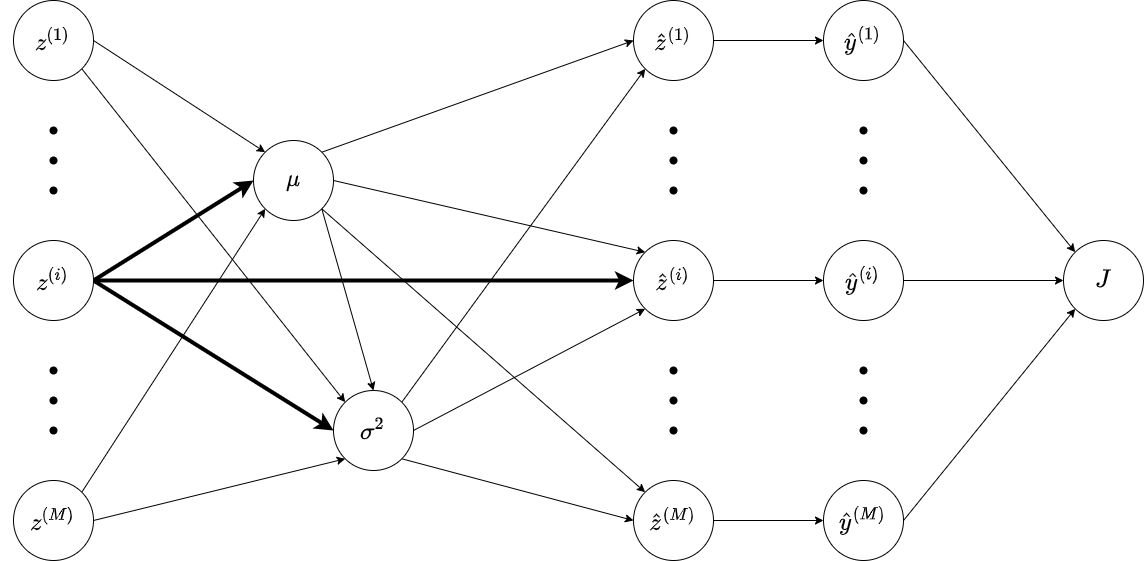
\includegraphics[scale=0.4]{Batch Norm dependencies graph.drawio.png}
    \caption{Figure 2.1.0: Dependencies graph of $J$ with respect to $z^{(i)}$}
\end{figure}
\begin{figure}[!ht]
    \captionsetup{labelformat=empty}
    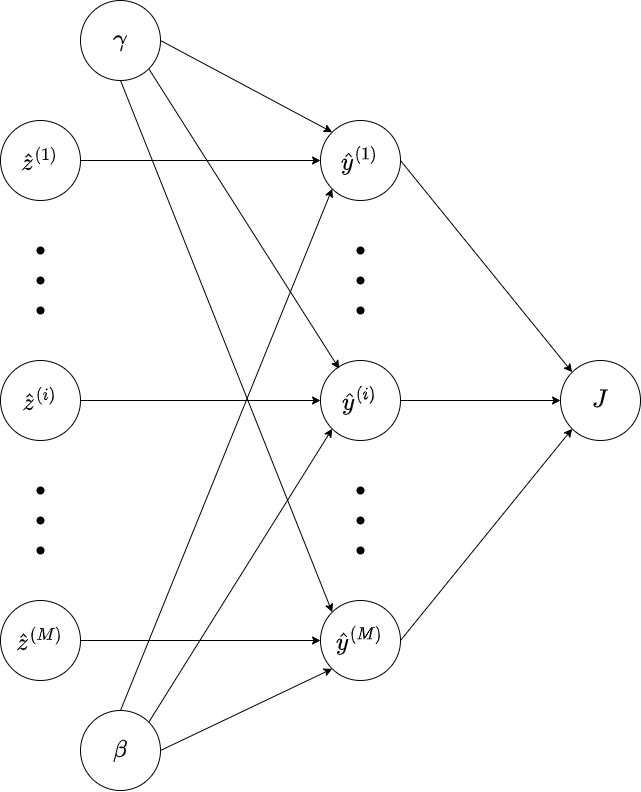
\includegraphics[scale=0.4]{Dependencies graph with beta gamma.drawio.png}
    \caption{Figure 2.1.1: Dependencies graph of $J$ with respect to $\boldsymbol{\gamma}$ and $\boldsymbol{\beta}$}  
\end{figure}
\begin{figure}
    \captionsetup{labelformat=empty}
    \centering
    \subfloat[\centering NN control]{{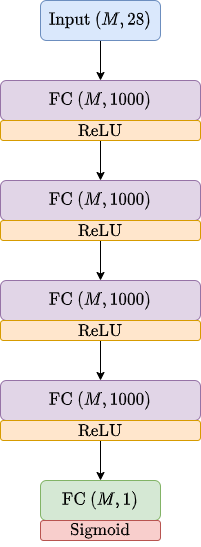
\includegraphics[scale=0.5]{NN regular.drawio.png} }}
    \qquad
    \subfloat[\centering NN with Batch Norm]{{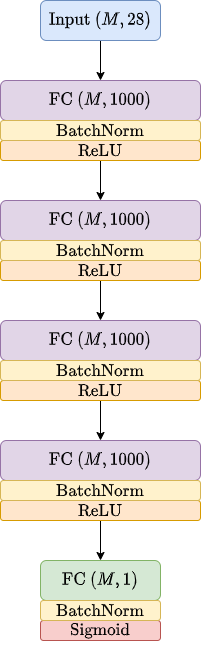
\includegraphics[scale=0.5]{NN batchnorm.drawio.png} }}
    \caption{Figure 3.1.0: The control model and the Batch Normalized model}
    \label{fig:example}
\end{figure}






\end{document}